% Chapter Chapter 9 For Reproducible Research in R and RStudio
% Christopher Gandrud
% Created: 16/07/2012 05:45:03 pm CEST
% Updated: 4 January 2012




\chapter{Showing Results with Tables}\label{TablesChapter}

Graphs and other visual methods, discussed in the next chapter, can often be a more effective way to present descriptive and inferential statistics than tables.\footnote{This is especially true of the small-print, high-density coefficient estimate tables that are sometimes descriptively called `train schedule' tables.} Nonetheless, tables of parameter estimates, descriptive statistics and so on can sometimes be an important tool for describing your data and presenting research findings. Learning how to dynamically connect statistical results with tables in your presentation documents aids reproducibility and can ultimately save you a lot of time.

Manually typing results into tables by hand is tedious, not very reproducible, and can introduce errors. It's especially tedious to retype tables to reflect changes you made to your data and models. Fortunately, you don't actually need to create tables by hand. There are many ways to have R do the work for you. 

The goal of this chapter is to learn how to dynamically create tables for you presentation documents written in LaTeX and Markdown. There are a number of ways to turn R objects into tables that can be dynamically included in LaTeX or Markdown/HTML markup. In this chapter we mostly focus on the \emph{xtable}\index{xtable} \cite[]{R-xtable} and \emph{apsrtable}\index{apsrtable} packages \cite[]{R-apsrtable}. \emph{xtable} can create tables for both of LaTeX and Markdown/HTML. \emph{apsrtable} usually produces publication quality tables more easily than \emph{xtable}. Unfortunately it only works with LaTeX and is less flexible with objects of classes it does not support.\footnote{These are not the only means available in R for creating presentation document tables from R objects. Others include the \emph{tables} \citep{R-tables},\index{table, R package} \emph{memisc} \citep{R-memisc}\index{memisc, R package} and \emph{estout} \citep{estout} packages as well as Paul Johnson's \texttt{outreg} function (see: \url{http://pj.freefaculty.org/R/WorkingExamples/outreg-worked.R}).} As we will learn at the end of the chapter, \texttt{knitr} allows us to dynamically incorporate tables from both packages into our documents.

\textbf{Warning:} Automating table creation removes the possibility of adding errors to your analyses by incorrectly copying output, a big potential problem in hand-created tables. However, it is not error free. You could easily create inaccurate tables through coding errors. So, as always, it is important to `eyeball' the output. Does it make sense? If you select a couple values in the R output do they match what is in the presentation document's table? If not, you need to go back to the code and see where things have gone wrong. With that caveat, let's start making tables.

\section{Table Basics}

Before getting into the details of how to create tables from R objects we need to first learn how generic tables are created in LaTeX and Markdown/HTML. If you are not familiar with basic LaTeX or Markdown syntax you might want to skip ahead to chapters \ref{LatexChapter} and \ref{MarkdownChapter}, respectively, before coming back to learn about making tables in these languages.

\subsection{Tables in LaTeX}\index{LaTeX tables}

Tables in LaTeX are usually embedded in two environments:\index{LaTeX table environment} the \texttt{table} and \texttt{tabular} environments. Before discussing these particular environments, what is a LaTeX environment in general?

A LaTeX environment is a part of the markup where special commands are executed. A simple environment is the \texttt{center} environment.\footnote{For a comprehensive list of LaTeX environments see: \url{http://latex.wikia.com/wiki/List_of_LaTeX_environments}.} Every thing typed in a center environment is, unsurprisingly, centered. If we typed:

\begin{knitrout}
\definecolor{shadecolor}{rgb}{0.969, 0.969, 0.969}\color{fgcolor}\begin{kframe}
\begin{alltt}
\textbackslash{}begin\{center\}
    This is a center environment.
\textbackslash{}end\{center\}
\end{alltt}
\end{kframe}
\end{knitrout}


\noindent We would create the following text in the PDF output:

\begin{center}
    This is a center environment.
\end{center}

\noindent LaTeX environments all follow the same general syntax:

\begin{knitrout}
\definecolor{shadecolor}{rgb}{0.969, 0.969, 0.969}\color{fgcolor}\begin{kframe}
\begin{alltt}
\textbackslash{}begin\{ENVIRONMENT_NAME\}
    . . .
    . . .
\textbackslash{}end\{ENVIRONMENT_NAME\}
\end{alltt}
\end{kframe}
\end{knitrout}


\noindent You do not have to indent the contents of an environment. Indentations neither affect how the document is compiled nor show up in the final PDF.\footnote{An aside: the \texttt{tabbing}\footnote{tabbing, LaTeX environment} environment is a useful way to create tabbed text in LaTeX. We don't cover this here.} It is conventional to indent them, however, because it makes the markup easier to read.

In this chapter we will learn about two types of environments you need for tables in LaTeX. The \texttt{tabular} environment allows you to format the content of a table. The \texttt{table} environment allows you to format a table's location in the text and its caption.

\paragraph{The \texttt{tabular} environment}\index{tabular, LaTeX environment}

The \texttt{tabular} environment allows you to create tables in LaTeX. Let's work through the basic syntax for a simple table.\footnote{For a comprehensive overview see the LaTeX Wiki page on tables: \url{http://en.wikibooks.org/wiki/LaTeX/Tables}.} 

To begin a simple tabular environment type \verb|\begin{tabular}{TABLE_SPEC}|. The \verb|TABLE_SPEC| argument allows you to specify the number of columns in a table and the alignment of text in each column. For example, to create a table with three columns, the first of which is left-justified and the latter two are center-justified we would type:

\begin{knitrout}
\definecolor{shadecolor}{rgb}{0.969, 0.969, 0.969}\color{fgcolor}\begin{kframe}
\begin{alltt}
\textbackslash{}begin\{tabular\}\{l c c\}
\end{alltt}
\end{kframe}
\end{knitrout}


\noindent The \texttt{l} argument creates a left-justified column, \texttt{c} creates a centered one. If we wanted a right-justified column we would use \texttt{r}.\footnote{You can also specify a column's width by using \texttt{m\{WIDTH\}} instead. This will create a column of a specified width that is vertically justified in the middle. For example, \texttt{p\{3cm\}} would create a column with a width of 3 centimeters. Text in the column would automatically be wrapped onto multiple lines if need be. You can replace the \texttt{m} with either \texttt{p} or \texttt{b}. \texttt{p} vertically aligns the text at the top, \texttt{b} aligns it at the bottom.} Finally we can add a horizontal line between columns by adding a vertical bar \texttt{|} between the columns arguments.\footnote{If you add two vertical bars (\texttt{||}) you will get two lines.} For example, to place a vertical line between the first and second column in our example table we would type:

\begin{knitrout}
\definecolor{shadecolor}{rgb}{0.969, 0.969, 0.969}\color{fgcolor}\begin{kframe}
\begin{alltt}
\textbackslash{}begin\{tabular\}\{l | c c\}
\end{alltt}
\end{kframe}
\end{knitrout}


Now let's enter content into our table. We saw earlier how CSV files delimit individual columns with commas. In LaTeX's \texttt{tabular} environment columns are delimited with ampersands (\verb|&|).\footnote{If you want to include an ampersand in the text of your LaTeX document you need to escape it like this: \texttt{\textbackslash{}\&}.}\index{ampersand in LaTeX} In CSV tables new lines are delimited by starting a new line. In LaTeX tables you use two backslashes (\verb|\\|).\footnote{You can use two backslashes outside of the \texttt{tabular} environment as well to force a new line. Also, to increase the space between the line you can add a vertical width argument to the double back slashes. For example, \texttt{\textbackslash{}\textbackslash{}[0.3cm]} will give you a three centimeter gap between the current line and the next one.} Here is a simple example of the first two lines of a table:

\begin{knitrout}
\definecolor{shadecolor}{rgb}{0.969, 0.969, 0.969}\color{fgcolor}\begin{kframe}
\begin{alltt}
\textbackslash{}begin\{tabular\}\{l | c c\}
    Observation & Variable1 & Variable2 \textbackslash{}\textbackslash{}
    Subject1 & a & b \textbackslash{}\textbackslash{}
\end{alltt}
\end{kframe}
\end{knitrout}


\noindent It is common to demarcate the row with a table's column names--the first row--with horizontal lines. A horizontal line also often demarcates a table's end. You can add horizontal in the \texttt{tabular} environment with the \verb|\hline| command.\footnote{The \texttt{\textbackslash{}hline} command works outside of the \texttt{tabular} environment as well.}

\begin{knitrout}
\definecolor{shadecolor}{rgb}{0.969, 0.969, 0.969}\color{fgcolor}\begin{kframe}
\begin{alltt}
\textbackslash{}begin\{tabular\}\{l | c c\}
    \textbackslash{}hline
    Observation & Variable1 & Variable2 \textbackslash{}\textbackslash{}
    \textbackslash{}hline \textbackslash{}hline
    Subject1 & a & b \textbackslash{}\textbackslash{}
    \textbackslash{}hline
\end{alltt}
\end{kframe}
\end{knitrout}


\noindent Finally, we close the \texttt{tabular} environment with \verb|\end{tabular}|. The full code (with a few extra rows added) is:

\begin{knitrout}
\definecolor{shadecolor}{rgb}{0.969, 0.969, 0.969}\color{fgcolor}\begin{kframe}
\begin{alltt}
\textbackslash{}begin\{tabular\}\{l | c c\}
    \textbackslash{}hline
    Observation & Variable1 & Variable2 \textbackslash{}\textbackslash{}
    \textbackslash{}hline \textbackslash{}hline
    Subject1 & a & b \textbackslash{}\textbackslash{}
    Subject2 & c & d \textbackslash{}\textbackslash{}
    Subject3 & e & f \textbackslash{}\textbackslash{}
    Subject4 & g & h \textbackslash{}\textbackslash{}
    \textbackslash{}hline
\textbackslash{}end\{tabular\}
\end{alltt}
\end{kframe}
\end{knitrout}


\noindent This produces the following table:

\begin{tabular}{l | c c}
    \hline
    Observation & Variable1 & Variable2 \\
    \hline \hline
    Subject1 & a & b \\
    Subject2 & c & d \\
    Subject3 & e & f \\
    Subject4 & g & h \\
    \hline
\end{tabular}

\paragraph{Table float environment}\index{table, LaTeX environment}

You might notice that the table we created so far lacks a title and is bunched very closely to the surrounding text. In LaTeX we can create a \texttt{table} float environment\index{float, LaTeX} to solve this problem. Float environments allow us to separate a table form the text, specify its location, and give it a caption.\footnote{We will see in the next chapter how to use \texttt{figure} floats as well.} To begin a \texttt{table}float environment use \verb|\begin{table}[POSITION_SPEC]|. The \verb|POSITION_SPEC| argument allows us to determine the location of the table. I can be set to \texttt{h} for here, i.e. where the table is written in the text. It can also be \texttt{t} to place it on the top of a page or \texttt{b} for the bottom of the page. To set a title for the table use the \verb|\caption| command.\index{caption, LaTeX command} LaTeX automatically determines the table's number, so you only need to enter the text. You can also declare a cross-reference key for the table with the \verb|\label| command.\footnote{This command works throughout LaTeX. To reference the table type in the text of your document \texttt{\textbackslash{}ref{KEY}}, where \texttt{KEY} is what you set with the \texttt{\textbackslash{}label} command. Use \texttt{\textbackslash{}pageref}\index{pageref, LaTeX command} to reference the page number.}\index{label, LaTeX command} A \texttt{table} environment is of course closed with \verb|\end{table}|. Let's see a full example.

\begin{knitrout}
\definecolor{shadecolor}{rgb}{0.969, 0.969, 0.969}\color{fgcolor}\begin{kframe}
\begin{alltt}
\textbackslash{}begin\{table\}[t]
    \textbackslash{}caption\{Example Simple LaTeX Table\}
    \textbackslash{}label\{ExLaTeXTable\}
    \textbackslash{}begin\{center\}
        \textbackslash{}begin\{tabular\}\{l | c c\}
            \textbackslash{}hline
            Observation & Variable1 & Variable2 \textbackslash{}\textbackslash{}
            \textbackslash{}hline \textbackslash{}hline
            Subject1 & a & b \textbackslash{}\textbackslash{}
            Subject2 & c & d \textbackslash{}\textbackslash{}
            Subject3 & e & f \textbackslash{}\textbackslash{}
            Subject4 & g & h \textbackslash{}\textbackslash{}
            \textbackslash{}hline
        \textbackslash{}end\{tabular\}
    \textbackslash{}end\{center\}
\textbackslash{}end\{table\}
\end{alltt}
\end{kframe}
\end{knitrout}


\begin{table}[t]
    \caption{Example Simple LaTeX Table}
    \label{ExLaTeXTable}
    \begin{center}
        \begin{tabular}{l | c c}
            \hline
            Observation & Variable1 & Variable2 \\
            \hline \hline
            Subject1 & a & b \\
            Subject2 & c & d \\
            Subject3 & e & f \\
            Subject4 & g & h \\
            \hline
        \end{tabular}
    \end{center}
\end{table}

\noindent Notice that the \texttt{tabular} environment is further nested in the \texttt{center} environment. This centers the table while leaving the table's title left-justified. The final result is Table \ref{ExLaTeXTable}.

You can see how typing out a table in LaTeX gets very tedious very fast. For all but the simplest tables it is best to try to have R do the table making work for you.

\subsection{Tables in Markdown/HTML}\index{Markdown/HTML tables}

Now we will briefly look at the syntax for creating simple Markdown and HTML tables before turning to learning how to have R create these tables for us.

\paragraph{Markdown tables}\index{Markdown tables}

Markdown table syntax, as with all Markdown syntax is generally much simpler than LaTeX's tabular syntax. The markup is much more human readable. Nontheless, larger tables can still be tedious to create.

You do not need to declare any new environments to start creating a Markdown table. Just start typing. Columns are delimited in Markdown tables with a vertical bar (\texttt{|}). Rows are started with a new line. To indicate the head of the table--usually the row(s) containing the column names--separate it from the body of the table a row of dashes (e.g. \verb|----|). Here is an example based on the table we created in the previous section:

\begin{knitrout}
\definecolor{shadecolor}{rgb}{0.969, 0.969, 0.969}\color{fgcolor}\begin{kframe}
\begin{alltt}
Observation | Variable1  | Variable2 
----------- | ---------- | --------- 
Subject1    | a          | b        
\end{alltt}
\end{kframe}
\end{knitrout}


\noindent Note that it is not necessary to line up the vertical bars. You just need to have the same number of them on each row.

You can specify each columns text justification using colons on the dashed row. For example this code will create the center-right-right justified format we did previously (with a few extra rows thrown in):

\begin{knitrout}
\definecolor{shadecolor}{rgb}{0.969, 0.969, 0.969}\color{fgcolor}\begin{kframe}
\begin{alltt}
Observation | Variable1 | Variable2 
:---------- | :-------: | :-------: 
Subject1    | a         | b        
Subject2    | c         | d        
Subject3    | e         | f        
Subject4    | g         | c       
\end{alltt}
\end{kframe}
\end{knitrout}


\noindent To create a right-right justified column simply place a colon on the right side of the dashes. 

The ultimate look of a Markdown table is highly dependent on the CSS style file you are using (see Chapter \ref{MarkdownChapter} for how to change your CSS style file). The default RStudio CSS style file formats our table like this:

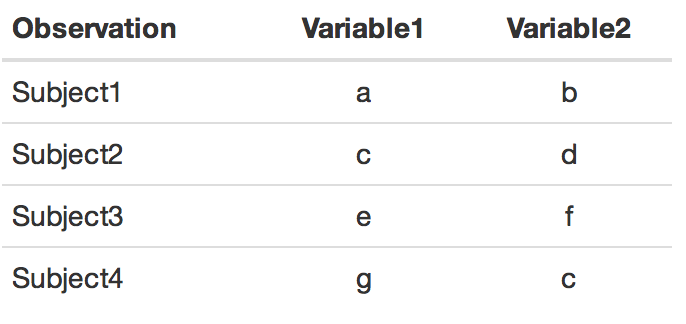
\includegraphics[scale = 0.6]{/git_repositories/Rep-Res-Book/Source/Children/Chapter9/images9/RStudioDefaultTableExample.png}

\noindent Using a different CSS style file\footnote{The table was created using the Upstanding Citizen style from the program Marked.\index{Marked}} we can get something like this:

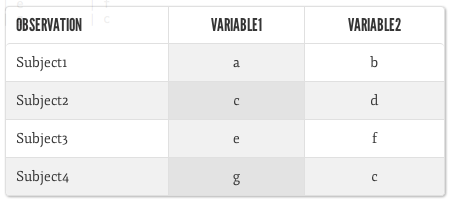
\includegraphics[scale = 0.6]{/git_repositories/Rep-Res-Book/Source/Children/Chapter9/images9/MarkedTableExample.png}

\noindent In basic Markdown you can add a caption with the heading syntax (see page \pageref{headings, Markdown}). For example:

\begin{knitrout}
\definecolor{shadecolor}{rgb}{0.969, 0.969, 0.969}\color{fgcolor}\begin{kframe}
\begin{verbatim}
### Example Simple Markdown Table
Observation | Variable1 | Variable2 
:---------- | :-------: | :-------: 
Subject1    | a         | b         
\end{verbatim}
\end{kframe}
\end{knitrout}


\noindent will produce something like this:

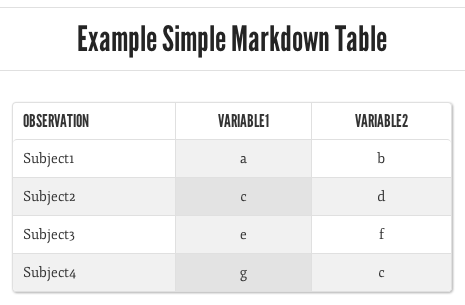
\includegraphics[scale = 0.6]{/git_repositories/Rep-Res-Book/Source/Children/Chapter9/images9/MarkedCaptionTableExample.png}

\noindent If you use MultiMarkdown you can use a more sophisticated caption by including the heading and cross reference key inside of square brackets (\verb|[]|) either directly before or directly after the table. Please see Chapter \ref{MarkdownChapter} (page \pageref{MultiMarkdownDiscussion}).

\paragraph{HTML tables}\index{HTML tables}

The \emph{xtable} package we will learn in the next section doesn't create tables formatted by Markdown syntax. It can creates tables with HTML syntax. This is useful for us because virtually any HTML markup can be incorporated into a Markdown document. In fact, Markdown table syntax is only a stepping stone for more easily producing tables with HTML syntax. So it is useful to understand the basic syntax for HTML tables.

HTML uses element ``tags''\index{element tag, HTML} to begin and end tables. The main element we use to create tables is, well the \texttt{tables} element. This is very similar to LaTeX's \texttt{tabular} environment. An HTML element generally begins with a start tag and ends with an end tag. Clearly this is very similar to LaTeX's \verb|\begin{}| and \verb|\end{}| commands. Begin tags are encapsulated in a greater than and less than sign and include the element tag name (\verb|<TAG>|). End tags are similar, but include a forward slash like this \verb|</TAG>|. The content of the element goes between the start and end tags. For example:

\begin{knitrout}
\definecolor{shadecolor}{rgb}{0.969, 0.969, 0.969}\color{fgcolor}\begin{kframe}
\begin{alltt}
<table>
    . . .
    . . .
</table>
\end{alltt}
\end{kframe}
\end{knitrout}


\noindent As in LaTeX you are not required to tab the content of a table element, however, it does make the markup document easier to read and, as the number of tags proliferates, easier to write.

You can add element attributes inside of start tags.\footnote{These work like arguments in R in that they change how the element is evaluated.} For example, to add a border to the table use: \verb|<table border="1">|.

Table rows are put inside of \texttt{tr}\index{tr, HTML element} (table rows) element tags. Individual cells are delimited with \texttt{td} (standard cell) tags.\index{td, HTML element} Here is what the first row of our example table looks like in basic HTML:

\begin{knitrout}
\definecolor{shadecolor}{rgb}{0.969, 0.969, 0.969}\color{fgcolor}\begin{kframe}
\begin{alltt}
<table>
    <tr>
        <td>Observation</td> <td>Variable1</td> <td><Variable2/td>
    </tr>
\end{alltt}
\end{kframe}
\end{knitrout}


\noindent We can further delimit a table's header row(s) from its body with the \texttt{thead} and \texttt{tbody} tags. Finally, before making a full table its useful to mention that table captions can be include with \texttt{caption} tags. Let's put this all together:

{\small
\begin{knitrout}
\definecolor{shadecolor}{rgb}{0.969, 0.969, 0.969}\color{fgcolor}\begin{kframe}
\begin{alltt}
<table>
    <thead>
        <tr>
            <td>Observation</td> <td>Variable1</td> <td>Variable2</td>
        </tr>
    </thead>
    <tbody>
        <tr>
            <td>Subject1</td> <td>a</td> <td>b</td>
        </tr>
        <tr>
            <td>Subject2</td> <td>c</td> <td>d</td>
        </tr>
        <tr>
            <td>Subject3</td> <td>e</td> <td>e</td>
        </tr>
        <tr>
            <td>Subject4</td> <td>f</td> <td>f</td>
        </tr>      
    </tbody>
</table>
\end{alltt}
\end{kframe}
\end{knitrout}

}

\noindent As with Markdown tables, the ultimate appearance of the table is highly dependent on the style files you use.

\section{Creating tables from R objects}

Just as the \texttt{read.csv} command turns an R data frame into a CSV formatted text file, there are a number of methods in R to take an object--e.g. a matrix, data frame, the output from a statistical analysis and so on--and turn them into LaTeX and HTML tables. In this section we will learn how to do this with the \emph{xtable} and \emph{apsrtable} packages.

\subsection{\emph{xtable} \& \emph{apsrtable} basics with supported class objects} 

The \emph{xtable} and \emph{apsrtable} packages are fairly easy to use if you want to convert a model object or an object of a class that they support into a table. To see a full list of object classes that \emph{xtable} supports type \texttt{methods(xtable)} into the R console after you have loaded the package. To see \emph{apsrtable}'s supported classes type \verb|showMethods("modelInfo")| into your console.

\subsubsection{\emph{xtable} for LaTeX}

Let's first look at how to create LaTeX tables with \emph{xtable}. Let's begin by creating a summary table of simple linear regression results using data from the \emph{swiss} data frame and R's \texttt{lm} (linear model) command.\index{lm} This data frame is included with R by default. The simple linear regression model we are going to make has the \emph{swiss} variable \textbf{Examination} as the dependent variable and \textbf{Education} as the only independent variable.\footnote{For a description of these variables type \texttt{?swiss} into the console}

















